\Chapter{Rest applikáció tesztelése}

\Section{Unit tesztek}

A fejlesztés során folyamatos logikai egység tesztek írása már fejlesztési időben jelentős mennyiségű tervezési és megvalósítással kapcsolatos hibára mutat rá.

A megvalósítás részeként a konfigurációs és kizárólag nyelvi elemeket tartalmazó osztályok kivételével, folyamatos tesztlefedettség ellenőrzéssel történt az implementáció.

\vskip 0.2in
A kódbázis, összesen 312 db egység tesztet tartalmaz, amelyek a mérések alapján 99\%-os tesztlefedettséget jelentenek.
Mint ahogy azt \aref{fig:jacocoReport} ábra is mutatja.

\begin{figure}[h]
\centering
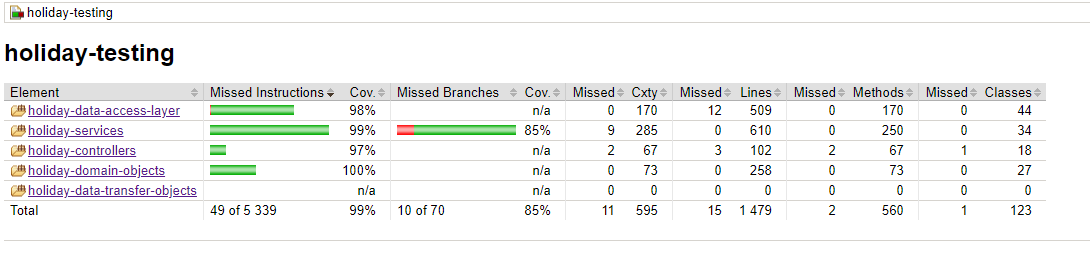
\includegraphics[scale=0.5]{images/jacocoReport.png}
\caption{Jacoco riport generált adatai.}
\label{fig:jacocoReport}
\end{figure}

Az alkalmazás teljes felépítése a tesztek futtatásával átlagosan 40 és 45 másodperc közé tehető.

\Section{Funkcionális tesztek Swagger UI segítségével}

A WEB applikációk szerver oldali logikája megjelenítési rétegtől függetlenül tesztelhetőek, az általunk létrehozott végpontok erre alkalmas programok segítségével és a megfelelő HTTP kérésekkel meghívhatóak és a program futási időben kiszolgálja azokat.
\vskip 0.2in

Ahhoz, hogy ne kelljen külső programot használni egy külső könyvtár segítségével saját felületet generálhatunk az végpontjaink számára. A kontextus épülésekor a külső függőség meghívódik és az általunk vezérlő típusként definiált osztályok HTTP hívással megjelölt függvényei alapján megjelenítést generál ami jól látható \aref{fig:swaggerUI}. 

\begin{figure}[h]
	\centering
	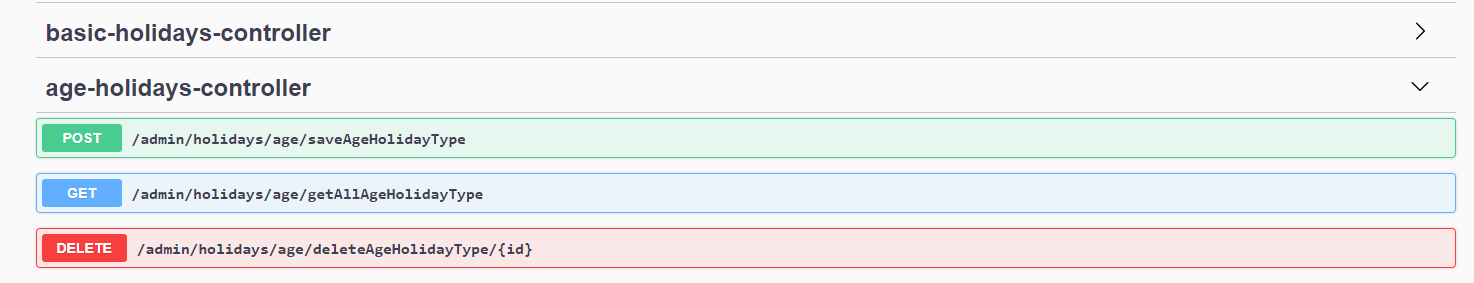
\includegraphics[scale=0.3]{images/swaggerUI.png}
	\caption{Swagger UI felület.}
	\label{fig:swaggerUI}
\end{figure}

Előnye, hogy nem csak láthatóvá teszi végpontokat, de dokumentációként is szolgál számunkra a bemeneti és visszatérési értékekről egyaránt. Továbbá biztosít még egy kitölthető űrlapot és egy mintát a aminek a segítségével a megfelelő JSON hívással ki is próbálhatjuk az adott funkció működését. 

A küldés \aref{fig:swaggerPostTest} ábrán \aref{fig:swaggerGetTest} pedig a lekérdezés tesztekése látható.

\begin{figure}[h]
	\centering
	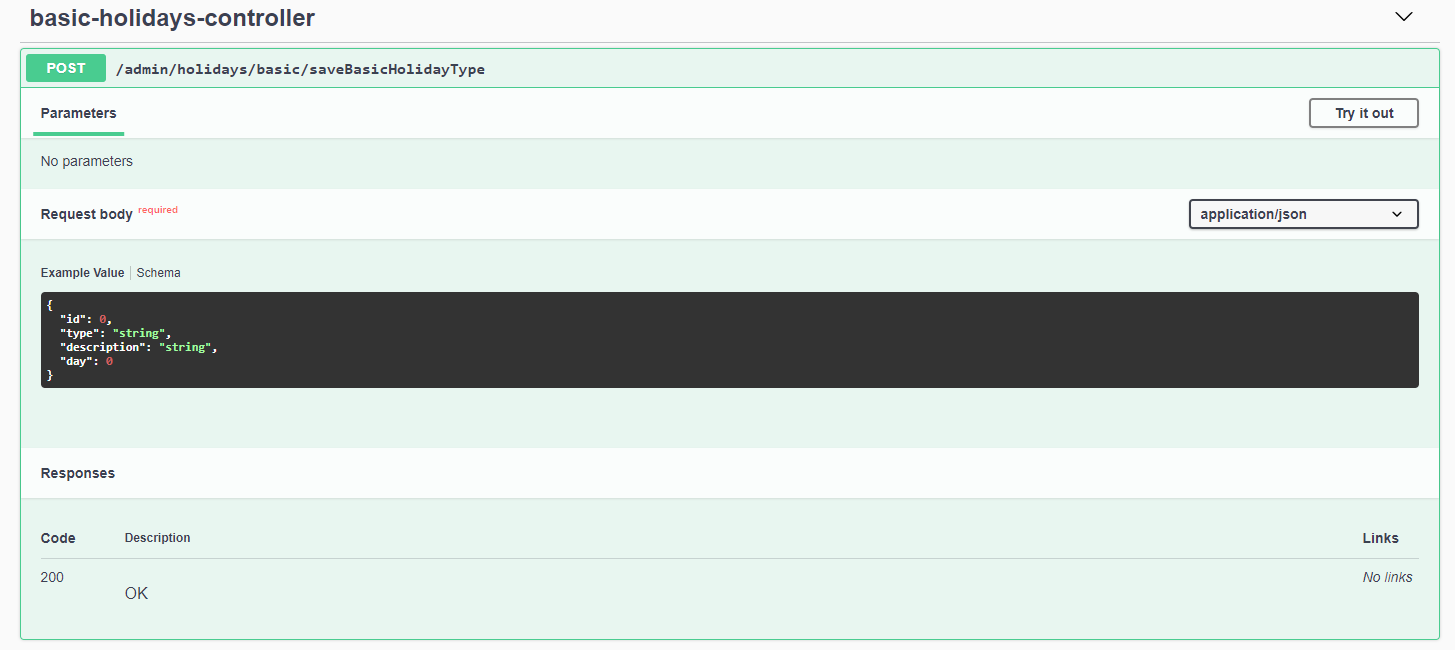
\includegraphics[scale=0.3]{images/swaggerPost.png}
	\caption{Swagger UI Post hívás tesztelése.}
	\label{fig:swaggerPostTest}
\end{figure}

\begin{figure}[h]
	\centering
	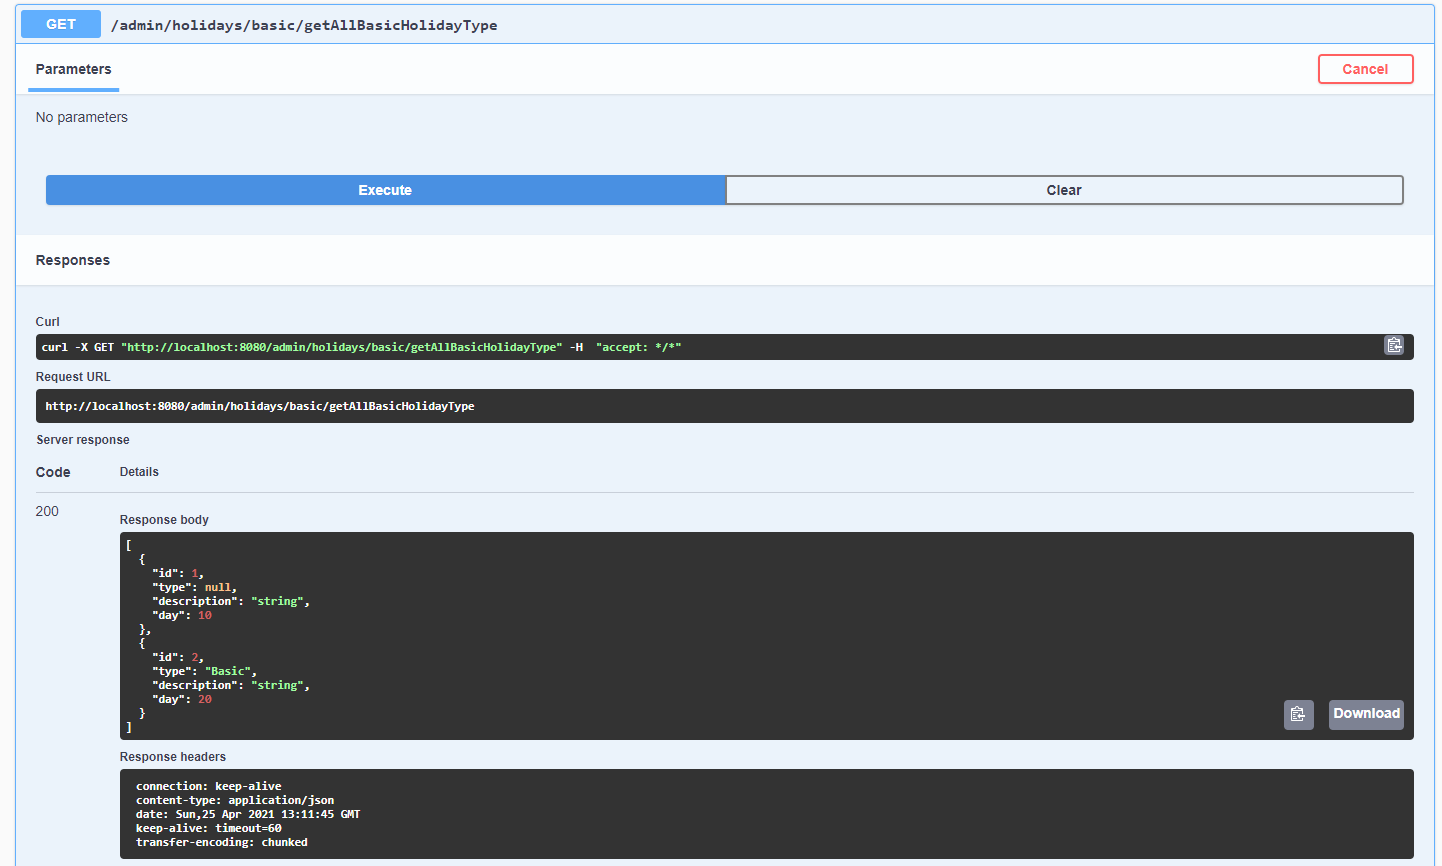
\includegraphics[scale=0.3]{images/swaggerGet.png}
	\caption{Swagger UI Get hívás tesztelése.}
	\label{fig:swaggerGetTest}
\end{figure}